\chapter{Marco Teórico}

Este capítulo va a poner en contexto al lector con respecto a conceptos básicos de criptografía para posteriormente explicar los algoritmos que van a ser implementados en el FPGA.\footnote{Según el ISO 7498-2 los términos correctos para encriptar y desencriptar son cifrar y descifrar respectivamente.}

\section{Conceptos Básicos}
Según la Real Academia Española \cite{bruce} la criptografía se define como 
\newline
\newline
\emph{Arte de escribir con clave secreta o de un modo enigmático.}
\newline
\newline
El mensaje que se desea transmitir es usualmente llamado \textit{texto plano} o simplemente \textit{mensaje}. Este mensaje pasa por un proceso donde se disfraza el texto plano en un \textit{texto cifrado}, el proceso es llamado \textit{cifrado}. El proceso inverso donde se toma un texto cifrado en un texto plano se denomina \textit{descifrado}. 

El texto plano o mensaje se denota usualmente por la letra M o P, el texto cifrado se denota usualmente por la letra C, la función o algoritmo que cifra se denota por E y la que descrifa se denota por D. Un algoritmo criptográfico corresponde a la función matemática para cifrar y descrifrar.
\newline
Se muestra en las Ecuaciones \ref{eqCifrado} y \ref{eqDescifrado} las relaciones entre estas notaciones. Note como al aplicarle la función de cifrado al texto plano se obtiene el texto cifrado y como al aplicarle la función de descifrado al texto cifrado se obtiene el texto plano. Finalmente se debe cumplir la identidad que describe la Ecuación \ref{eqCifraDescifra}. \cite{bruce}
\begin{equation} \label{eqCifrado}
E(M) = C
\end{equation}
\begin{equation} \label{eqDescifrado}
D(C) = M
\end{equation}
\begin{equation} \label{eqCifraDescifra}
D(E(M)) = M
\end{equation}


La importancia de criptografía transciende más allá de brindar la confidencialidad en la comunicación la criptografía también cumple con la siguientes tareas:
\begin{itemize}
\item Autenticación: El receptor del mensaje debe de poder conocer y asegurar el emisor del mensaje, esto para que un tercero no pueda adjudicarse la identidad del emisor.
\item Integridad: El receptor tiene que poder asegurarse que el mensaje no fue cambiado en el transito del mismo. Esto para que un tercero no pueda cambiar el contenido enviado por el emisor sin que el receptor lo sepa.
\item \textit{Non-repudiation}: El emisor del mensaje no puede negar que el mensaje fue enviado por él. 
\end{itemize}

\section{Sistema criptográfico (\textit{criptosistema})}
Cuando la seguridad del algoritmo se basa en como procede el algoritmo, se denomina \textit{algoritmo restringido}. Este tipo de algoritmos son poco utilizados en la actualidad debido al gran problema que presentan. Tomemos de ejemplo que un grupo de usuarios decide utilizar un algoritmo de cifrado restringido para sus comunicaciones, se tendrá una comunicación segura hasta que alguno de los miembros decida salirse del grupo, ya que el usuario al no pertenecer más al grupo, no le importa mantener en secreto el algoritmo y puede distribuirlo para que terceros intercepen las comunicaciones. Así cada vez que un miembro deja el grupo, el grupo debe proceder a cambiarse a todo un nuevo algoritmo lo cual puede tornarse una labor complicada.

En cambio la criptografía moderna \cite{denning} agrega el concepto de \textit{llave} donde se tiene un algoritmo el cual toma como parámetro de entrada una llave y el texto plano o texto cifrado y cifra o descifra el mismo de forma correcta únicamente si se tiene la llave correcta. Retomando el ejemplo anterior, el grupo solamente necesitaría cambiar de llave cuando un miembro se va, facilitando el uso del cifrado y manteniendo las comunicaciones secretas.

Este concepto anterior viene a definir lo que actualmente se conoce como sistema criptográfico o \textit{criptosistema}. Según \cite{denning} un criptosistema cuenta con 5 componentes:
\begin{itemize}
\item Un espacio de textos planos o mensajes ($M$)
\item Un espacio de textos cifrados ($C$)
\item Un espacio de llaves ($k$)
\item Una familia de \textit{transformaciones de cifrado}: $E_K: M\rightarrow C$ donde $K \epsilon  k$
\item Una familia de \textit{transformaciones de descrifrado}: $C_K: C\rightarrow M$ donde $K \epsilon  k$
\end{itemize} 


Se entiende como \textit{espacio} el conjunto de posibles valores para la variable dada, sea esta M, C o K.
Y una familia de transformaciones corresponde a todos los posibles mapeos que se pueden realizar de un espacio a otro (de $M$ a $C$ o viceversa) con todos los valores contenidos en el espacio $k$.

\begin{figure}
	\centering
	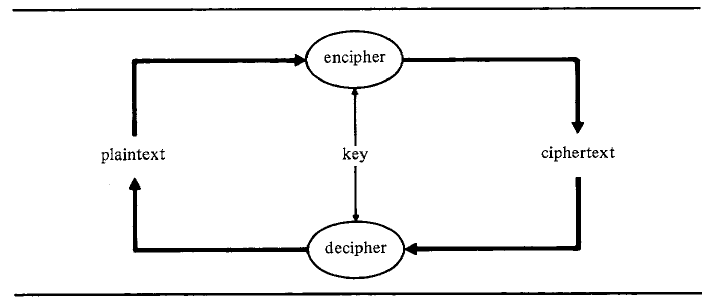
\includegraphics[width=0.8\textwidth]{./images/figExplicacionSistemaCripto}
	\caption{Descripción gráfica de un sistema criptográfico.}
	\label{figExplicacionSistemaCripto}
\end{figure}


En la actualidad se trabaja la criptografía sobre computadoras, es decir, cifrando y descrifrando bits, los cuales pueden tener diferentes significados, ya sea una imagen, un texto, un programa, etc. Esto significa que en la actualidad no se trabaja sobre caracteres del alfabeto o símbolos, sino más bien sobre 1's y 0's. Esto toma relevancia ya que al tener solo dos símbolos para cifrar, los algoritmos se vuelven más complejos por la falta de alternativas para sustituir un símbolo por otro.

Así antiguamente la criptografía se basaba en caracteres que eran sustituidos o traspuestos por otros caracteres. Esto corresponde a cifrados de sustitución y de transposición, los cuales continúan siendo la base de la criptografía pero basado los 2 símbolos del sistema binario.

Como se explicó anteriormente este tipo de cifrado se basa en tomar un caracter del texto plano y sustituirlo por otro caracter. Para descrifrar el texto cifrado simplemente se sustituyen de vuelta los caracteres y listo.

Según \cite{bruce} en la criptografía clásica existen 4 tipos de cifrado por sustitución:
\begin{itemize}
\item Cifrado de sustitución simple: Una sustitución de uno a uno entre cada caracter del texto plano y el texto cifrado.
Ejemplos de este tipo de sustitución son el famoso cifrado de César y el ROT13 utilizado en UNIX.

\item Cifrado de sustitución homofónico: Una sustición de uno a muchos. Un caracter del texto plano, por ejemplo A, puede ser sustituido por varios caracteres en el texto crifado, por ejemplo ``5'', ``13'', ``43''. Observe la Figura \ref{figExampleHomophonicCipher} donde se presenta una serie de posibles asignaciones de números a las letras del mensaje PLAIN PILOT y un posible texto cifrado haciendo uso de este tipo de cifrado.

\begin{figure}
	\centering
	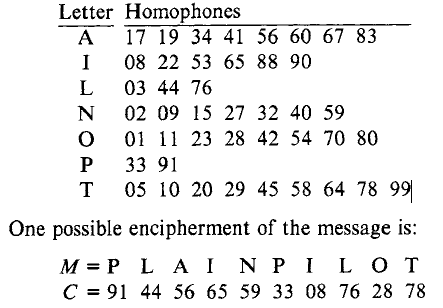
\includegraphics[width=0.6\textwidth]{./images/figExampleHomophonicCipher}
	\caption{Ejemplo de cifrado homofónico.}
	\label{figExampleHomophonicCipher}
\end{figure}


\item Cifrado de sustitución de poligrama: Una sustitución por bloques en donde se toma un bloque de caracteres del texto plano y se sustituye por su bloque equivalente en el texto cifrado. Por ejemplo si en el texto plano se tiene ``ABC'' se sustituye por ``SLL'' en el texto cifrado.

\item Cifrado de sustitución polialfabético: ????? 
\end{itemize}

La otra variedad de algoritmos son los de tranposición, en este tipo de algoritmos de cifrado el texto plano se convierte en texto cifrado cuando el orden de los caracteres es cambiado bajo alguna norma. Un ejemplo moderno de este tipo de algoritmos es el ``rail-fence" donde el texto plano se reacomoda con la forma de una cerca como se observa en la Figura \ref{figExampleTranspositionCipher}. En este caso la llave del algoritmos sería la profundidad de la cerca, para efectos de este ejemplo es de 3.

\begin{figure}
	\centering
	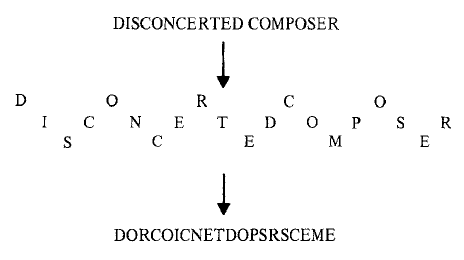
\includegraphics[width=0.65\textwidth]{./images/figExampleTranspositionCipher}
	\caption{Ejemplo de cifrado de transposición.}
	\label{figExampleTranspositionCipher}
\end{figure}


Actualmente en los algoritmos que se implementan en computadoras se combina tanto la tranposición como la sustitución. Por ejemplo se tiene el algoritmo RC5, el cual se desarrollará más adelante en este proyecto en donde se utiliza corrimientos o rotaciones a bits (tranposición) y sumas o XOR's (sustituciones) para cifrar el texto plano. Los algoritmos que se implementan en la criptografía se dividen en 2 categorías principales: simétricos y de llave pública (también llamados asimétricos \cite{???}).


\section{Algoritmos de cifrado}
\subsection{Algoritmos simétricos}
\cite{bruce} da una muy buena analogía para explicar el concepto de un algoritmo simétrico. Piense en el algoritmo como una caja fuerte. La combinación de la caja fuerte vendría a ser la \textit{llave} del algoritmo. Note como en una caja fuerte cualquier persona con la combinación puede llegar, abrir la caja y poner o sacar documentos de la misma. En el caso de no conocer la combinación, se debe proceder a forzar la caja o probando todas las combinaciones posibles hasta hallar la correcta. Es decir en un algoritmo simétrico se cuenta con una llave única que funciona tanto para cifrar como para descrifrar los mensajes como se muestra en la Figura \ref{figSimmetricKeyAlgorithm}. La notación para el cifrado y descrifado en estos algoritmos se muestra en las Ecuaciones \ref{eqCifradoSimetrico} y \ref{eqDescifradoSimetrico}.
\begin{equation}\label{eqCifradoSimetrico}
E_K (M) = C
\end{equation}

\begin{equation}\label{eqDescifradoSimetrico}
D_K (C) = M
\end{equation}


\begin{figure}
	\centering
	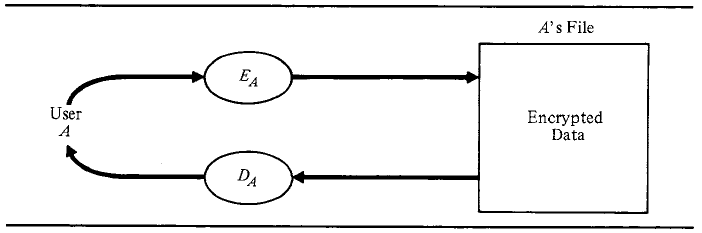
\includegraphics[width=0.9\textwidth]{./images/figSimmetricKeyAlgorithm}
	\caption{Descripción gráfica de una algoritmo de llave simétrica.}
	\label{figSimmetricKeyAlgorithm}
\end{figure}


Los algoritmos simétricos se dividen en 2 categorías (\cite{bruce}):

\begin{itemize}
\item cifrado de bloque: Se cifra en bloques de bits ya sea bytes, words, etc. Es decir cuando se va a proceder a cifrar un texto plano, se segmenta el texto en grupos de bits y estos son cifrados de manera independiente. Se puede tomar como ejemplo el algoritmo \textit{Data Encryption Standart} (DES) el cual cifra sobre bloques de 64 bits.

\item cifrado de \textit{Stream}: Es cuando se trabaja sobre un bit únicamente. Estos no son muy usuales en la actualidad ya que al trabajar en lenguaje binario solo se cuenta con 2 símbolos y si se cifra únicamente un bit no existen muchas posibilidades para sustituir o transposicionar.
\end{itemize}

Según (\cite{bruce}) los criptosistemas simétricos en la red afrontan los siguientes problemas
\begin{itemize}
\item Distribución de la llave: La llave se debe mantener en secreto. Esto en la actualidad en una tarea demasiado díficil de lograr porque la llave debe ser conocida para el cifrado y descifrado (emisores y receptores) entonces para establecer una comunicación segura el primer paso debe ser entregar la llave de forma segura, lo cual en una red de computadoras se puede tornar una tarea prácticamente imposible de realizar. La única solución sería entregar las llaves mediantes un servicio de \textit{courier} o similares e igualmente se corren riesgos. 

\item Compromiso de seguridad: Si la llave es conocida por un tercero, si este intercepta el tráfico de información, todas las comunicaciones serán descifradas fácilmente.

\item Comunicaciones aisladas: En el caso de que cada usuario de una red se desee comunicar secretamente por separado con todos los otros usuarios del misma haciendo uso del mismo criptosistema, se debe utilizar una llave diferente para cada comunicación. Así para una red de N usuarios se requieren $N(N - 1)/2$ llaves. A primera vista esto no parece tan importante pero por ejemplo para 10 usuarios, se necesitan 45 llaves lo cual está bien, pero para 100 usuarios se necesitarían 4950 llaves.
\end{itemize}



\subsection{Algoritmos de llave pública}
Nuevamente \cite{bruce} nos ofrece una excelente analogía para explicar en este caso los algoritmos de llave pública. Tenemos un \textit{mailbox}, donde cualquier persona puede poner un mensaje adentro pero ÚNICAMENTE el dueño puede abrirlo para sacar y leer los mensajes.
\newline
\newline
En los algoritmos de llave pública los emisores hacen uso de una llave para cifrar los mensajes que desean enviar pero estos mensajes pueden ser descrifrados únicamente si se tiene la llave para descifrar mensajes que es diferente de la llave para cifrar, la cual la tendrá el receptor bien resguardada. En la Figura \ref{figPublicKeyAlgorithm} se muestra el diagrama básico de un algoritmo de llave pública.

\begin{figure}
	\centering
	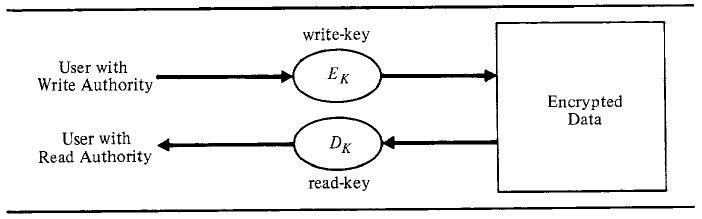
\includegraphics[width=0.65\textwidth]{./images/figPublicKeyAlgorithm}
	\caption{Descripción gráfica de una algoritmo de llave pública.}
	\label{figPublicKeyAlgorithm}
\end{figure}

Estos algoritmos sientan su base matemática en funciones llamadas \textit{one-way} en donde al aplicarle una función a una variable, la variable no puede retornar a su valor original de ninguna manera, es decir la función no tiene una inversa. 

Según \cite{bruce} existen funciones \textit{one-way} con una ``puerta trasera'' donde se puede retornar a la variable original, este tipo de funciones son las que se implementan en algoritmos de llave pública.

En estos algoritmos no es posible a partir de la llave para cifrar obtener la llave para descrifrar. Esto permite que la llave para cifrar se pueda hacer pública, por lo cual recibe el nombre de llave pública y la llave para descrifrar se denomina llave privada. La notación para estos algoritmos corresponde a la de las Ecuaciones \
\begin{equation} \label{eqCifradoPublico}
E_K_1 (M) = C
\end{equation}
\begin{equation} \label{eqDescfiradoPublico}
D_K_2 (C) = M
\end{equation}

El objetivo de utilizar cifrado de llave pública se basa en:
\begin{itemize}
\item Receptor y emisor acuerdan un sistema de cifrado.
\item El receptor entrega al emisor su llave pública.
\item El emisor cifra el texto plano haciendo uso de la llave pública entregada y el sistema acordado.
\item El emisor envía el texto cifrado.
\item El receptor descrifa el texto cifrado haciendo uso de la llave privada.
\end{itemize}


De esta manera no hay forma que fisgones logren descrifrar el mensaje aunque obtengan la llave pública, así el receptor se asegura que las comunicaciones van a ser mucho más seguras ya que el emisor deja de tener la llave para descifrar y así no puede brindarse a nadie o que sea robada a este.



Before, Alice and Bob had to agree on a key in
secret. Alice could choose one at random, but she still had to get it to Bob. She
could hand it to him sometime beforehand, but that requires foresight. She
could send it to him by secure courier, but that takes time

More commonly, a network of users agrees on a public-key cryptosystem.
Every user has his or her own public key and private key, and the public keys
are all published in a database somewhere. Now the protocol is even easier:
(1) Alice gets Bob’s public key from the database.
(2) Alice encrypts her message using Bob’s public key and sends it to
Bob.
(3) Bob then decrypts Alice’s message using his private key.











// Hybrid cryptosystems
In the real world, public-key algorithms are not a substitute for symmetric
algorithms. They are not used to encrypt messages; they are used to encrypt
keys. There are two reasons for this:
1. Public-key algorithms are slow. Symmetric algorithms are generally
at least 1000 times faster than public-key algorithms. Yes, computers
are getting faster and faster, and in 15 years computers will be able to do
public-key cryptography at speeds comparable to symmetric
cryptography today. But bandwidth requirements are also increasing,
and there will always be the need to encrypt data faster than public-key
cryptography can manage.
2. Public-key cryptosystems are vulnerable to chosen-plaintext attacks.
If C = E(P), when P is one plaintext out of a set of n possible plaintexts,
then a cryptanalyst only has to encrypt all n possible plaintexts and
compare the results with C (remember, the encryption key is public). He
won’t be able to recover the decryption key this way, but he will be able
to determine P.


In most practical implementations public-key cryptography is used to secure
and distribute session keys; those session keys are used with symmetric
algorithms to secure message traffic [879]. This is sometimes called a hybrid
cryptosystem.
(1) Bob sends Alice his public key.
(2) Alice generates a random session key, K, encrypts it using Bob’s
public key, and sends it to Bob.
EB(K)
(3) Bob decrypts Alice’s message using his private key to recover the
session key.
DB(EB(K)) = K
(4) Both of them encrypt their communications using the same session
key.
Using public-key cryptography for key distribution solves a very important
key-management problem. With symmetric cryptography, the data encryption
key sits around until it is used. If Eve ever gets her hands on it, she can decrypt
messages encrypted with it. With the previous protocol, the session key is
created when it is needed to encrypt communications and destroyed when it is
no longer needed. This drastically reduces the risk of compromising the
session key. Of course, the private key is vulnerable to compromise, but it is at
less risk because it is only used once per communication to encrypt a session
key. This is further discussed in Section 3.1.




































There are many cryptographic algorithms. These are three of the most common:

— DES (Data Encryption Standard) is the most popular computer encryption algorithm. DES is a U.S. and international standard. It is a
symmetric algorithm; the same key is used for encryption and decryption.

— RSA (named for its creators—Rivest, Shamir, and Adleman) is the most popular public-key algorithm. It can be used for both encryption
and digital signatures.

— DSA (Digital Signature Algorithm, used as part of the Digital Signature Standard) is another public-key algorithm. It cannot be used
for encryption, but only for digital signatures.





